% Created by tikzDevice version 0.10.1 on 2017-12-04 16:18:46
% !TEX encoding = UTF-8 Unicode
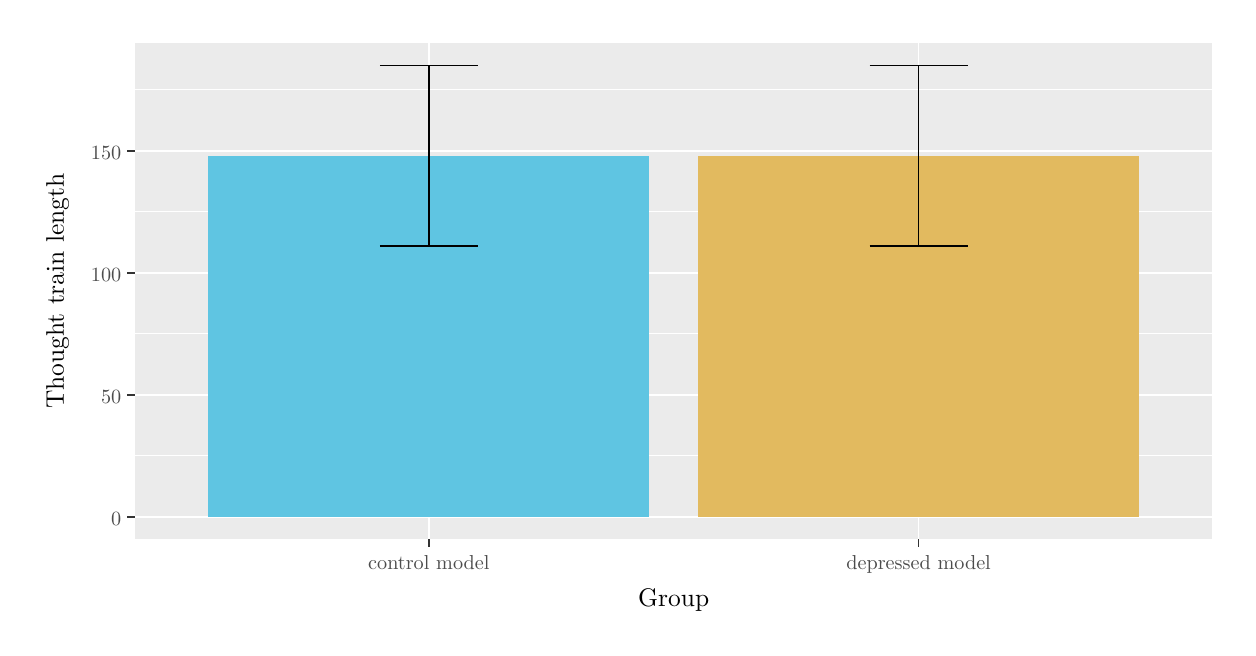
\begin{tikzpicture}[x=1pt,y=1pt]
\definecolor{fillColor}{RGB}{255,255,255}
\path[use as bounding box,fill=fillColor,fill opacity=0.00] (0,0) rectangle (433.62,216.81);
\begin{scope}
\path[clip] (  0.00,  0.00) rectangle (433.62,216.81);
\definecolor{drawColor}{RGB}{255,255,255}
\definecolor{fillColor}{RGB}{255,255,255}

\path[draw=drawColor,line width= 0.6pt,line join=round,line cap=round,fill=fillColor] (  0.00,  0.00) rectangle (433.62,216.81);
\end{scope}
\begin{scope}
\path[clip] ( 38.78, 31.92) rectangle (428.12,211.31);
\definecolor{fillColor}{gray}{0.92}

\path[fill=fillColor] ( 38.78, 31.92) rectangle (428.12,211.31);
\definecolor{drawColor}{RGB}{255,255,255}

\path[draw=drawColor,line width= 0.3pt,line join=round] ( 38.78, 62.11) --
	(428.12, 62.11);

\path[draw=drawColor,line width= 0.3pt,line join=round] ( 38.78,106.19) --
	(428.12,106.19);

\path[draw=drawColor,line width= 0.3pt,line join=round] ( 38.78,150.27) --
	(428.12,150.27);

\path[draw=drawColor,line width= 0.3pt,line join=round] ( 38.78,194.35) --
	(428.12,194.35);

\path[draw=drawColor,line width= 0.6pt,line join=round] ( 38.78, 40.07) --
	(428.12, 40.07);

\path[draw=drawColor,line width= 0.6pt,line join=round] ( 38.78, 84.15) --
	(428.12, 84.15);

\path[draw=drawColor,line width= 0.6pt,line join=round] ( 38.78,128.23) --
	(428.12,128.23);

\path[draw=drawColor,line width= 0.6pt,line join=round] ( 38.78,172.31) --
	(428.12,172.31);

\path[draw=drawColor,line width= 0.6pt,line join=round] (144.96, 31.92) --
	(144.96,211.31);

\path[draw=drawColor,line width= 0.6pt,line join=round] (321.94, 31.92) --
	(321.94,211.31);
\definecolor{fillColor}{RGB}{95,197,226}

\path[fill=fillColor] ( 65.33, 40.07) rectangle (224.60,170.50);
\definecolor{fillColor}{RGB}{226,186,95}

\path[fill=fillColor] (242.30, 40.07) rectangle (401.57,170.50);
\definecolor{drawColor}{RGB}{0,0,0}

\path[draw=drawColor,line width= 0.6pt,line join=round] (127.27,203.16) --
	(162.66,203.16);

\path[draw=drawColor,line width= 0.6pt,line join=round] (144.96,203.16) --
	(144.96,137.84);

\path[draw=drawColor,line width= 0.6pt,line join=round] (127.27,137.84) --
	(162.66,137.84);

\path[draw=drawColor,line width= 0.6pt,line join=round] (304.24,203.16) --
	(339.63,203.16);

\path[draw=drawColor,line width= 0.6pt,line join=round] (321.94,203.16) --
	(321.94,137.84);

\path[draw=drawColor,line width= 0.6pt,line join=round] (304.24,137.84) --
	(339.63,137.84);
\end{scope}
\begin{scope}
\path[clip] (  0.00,  0.00) rectangle (433.62,216.81);
\definecolor{drawColor}{gray}{0.30}

\node[text=drawColor,anchor=base east,inner sep=0pt, outer sep=0pt, scale=  0.73] at ( 33.83, 37.04) {0};

\node[text=drawColor,anchor=base east,inner sep=0pt, outer sep=0pt, scale=  0.73] at ( 33.83, 81.12) {50};

\node[text=drawColor,anchor=base east,inner sep=0pt, outer sep=0pt, scale=  0.73] at ( 33.83,125.20) {100};

\node[text=drawColor,anchor=base east,inner sep=0pt, outer sep=0pt, scale=  0.73] at ( 33.83,169.28) {150};
\end{scope}
\begin{scope}
\path[clip] (  0.00,  0.00) rectangle (433.62,216.81);
\definecolor{drawColor}{gray}{0.20}

\path[draw=drawColor,line width= 0.6pt,line join=round] ( 36.03, 40.07) --
	( 38.78, 40.07);

\path[draw=drawColor,line width= 0.6pt,line join=round] ( 36.03, 84.15) --
	( 38.78, 84.15);

\path[draw=drawColor,line width= 0.6pt,line join=round] ( 36.03,128.23) --
	( 38.78,128.23);

\path[draw=drawColor,line width= 0.6pt,line join=round] ( 36.03,172.31) --
	( 38.78,172.31);
\end{scope}
\begin{scope}
\path[clip] (  0.00,  0.00) rectangle (433.62,216.81);
\definecolor{drawColor}{gray}{0.20}

\path[draw=drawColor,line width= 0.6pt,line join=round] (144.96, 29.17) --
	(144.96, 31.92);

\path[draw=drawColor,line width= 0.6pt,line join=round] (321.94, 29.17) --
	(321.94, 31.92);
\end{scope}
\begin{scope}
\path[clip] (  0.00,  0.00) rectangle (433.62,216.81);
\definecolor{drawColor}{gray}{0.30}

\node[text=drawColor,anchor=base,inner sep=0pt, outer sep=0pt, scale=  0.73] at (144.96, 20.91) {control model};

\node[text=drawColor,anchor=base,inner sep=0pt, outer sep=0pt, scale=  0.73] at (321.94, 20.91) {depressed model};
\end{scope}
\begin{scope}
\path[clip] (  0.00,  0.00) rectangle (433.62,216.81);
\definecolor{drawColor}{RGB}{0,0,0}

\node[text=drawColor,anchor=base,inner sep=0pt, outer sep=0pt, scale=  0.92] at (233.45,  7.83) {Group};
\end{scope}
\begin{scope}
\path[clip] (  0.00,  0.00) rectangle (433.62,216.81);
\definecolor{drawColor}{RGB}{0,0,0}

\node[text=drawColor,rotate= 90.00,anchor=base,inner sep=0pt, outer sep=0pt, scale=  0.92] at ( 13.08,121.61) {Thought train length};
\end{scope}
\end{tikzpicture}
